\section{Design}\label{sect:design}
\subsection{System-level design}
The complete system consists of energy harvesting source, energy storage for times when harvesting energy is not possible, AC/DC and DC/DC converters for maintaining required voltage levels in different blocks of system, accelerometer for measuring the acceleration in tyre and radio/microcontroller module for transmitting the data. Figure \ref{fiq:system_block_diagram} shows the power and data flow between subsections of system. 


\begin{figure}[htb]
\begin{center}
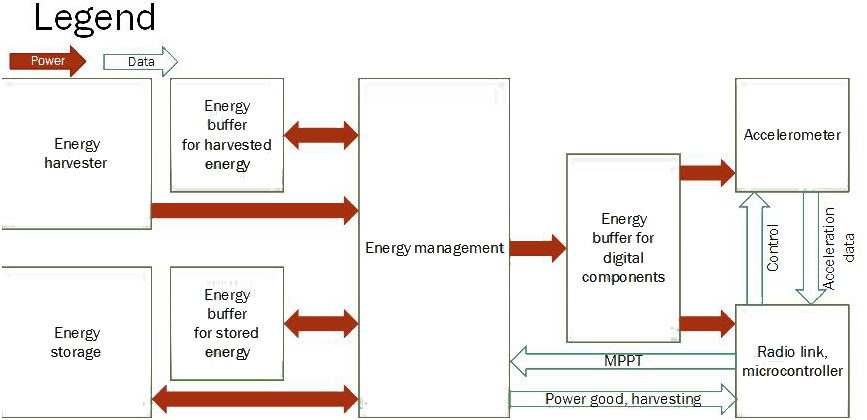
\includegraphics[width=\columnwidth]{images/own_dwg/system_block_diagram.jpg}
\end{center}
\caption{\label{fiq:system_block_diagram} Block diagram of a complete system. Harvested energy comes to system from top left, energy management system can charge storage when excess energy is available and use the stored energy when the harvested energy is insufficient for the system operation. On the right side is control logic and sensor. The experimental system has energy harvesting, energy storage and energy management sections, but control logic, radio comminication and sensing are outside the scope of the experimental work.}
\label{liitekuva}
\end{figure}

Energy harvester can use any suitable source presented in section \ref{sect:overview} for electrical energy. Energy management section rectifies AC voltage and buffers that rectified voltage on a capacitor. The energy storage can be a supercapacitor or a rechargeable battery. Both of these storage technologies can benefit from having an energy buffer in parallel to supply peak currents. Energy management circuitry chooses whether to use harvested energy or stored energy and regulates the energy to voltage level compatible with the system. Digital components require their own local power buffer capacitors to supply high-frequency currents required by megahertz clocks onboard these circuits.

Microcontroller is used to manage the application layer of system. The microcontroller can for example  send status updates over radio link more often if there is harvested energy available and reduce system power consumption when the system is running on a stored energy.

Next section presents details of expected power consumption and duty cycles for various components. A few components are selected to provide examples of required system power.

\subsection{Power requirements of a system} \label{sect:power_requirement}
The sensor system has three distinct states. One is sleeping, conserving power as much as possible while the car is not moving.
Second state is measuring, when the radio connection is off but electronics are active and gathering data.
Third state is transmitting, when the data is relayed to a drive computer in the car.

Energy and power consumption are estimated by reviewing a few suitable components and their power requirements. 
Energy management is handled by a specialised integrated circuit (IC), LTC3331 \cite{Technology}.

Communication is handled by a Bluetooth-low energy (BLE) module, which contains a general-purpose microcontroller for application flow control.
We use BLE113 \cite{Bluegiga2013} which is such a module.

Finally there is an accelerometer which is used for gathering data out of the system, ADXL375 \cite{ADXLDatasheet}. ADXL375 is a low-power digital accelerometer with dynamic range of 200 g. Table \ref{power_consumption_table}  summarises the estimated power requirement of each subsection of system. System level voltage is selected to be 2.5 V, as that is lowest voltage which LTC3331 can supply and which allows all devices to function. Lowest possible voltage is selected to reduce the power draw.

\begin{table}[htb]
\caption{\label{power_consumption_table} Current and power consumption of system at different activity levels. Power is calculated from current by multiplying current with 2.5 V.}
\begin{center}
\fbox{
\begin{tabular}{l l r r}
\textbf{Device}		& \textbf{Sleep} 	& \textbf{Monitoring}	& \textbf{Communicating}\\ \hline
LTC3331			& 0.2 $\mu A$		& 80 $\mu A$ 		& 6 675 $\mu A$ 		\\ 
BLE113			& 0.9 $\mu A$ 		& 275 $\mu A$ 		& 26 000 $\mu A$	\\ 
ADXL375			& 0.1 $\mu A$ 		& 140 $\mu A$ 		& 140 $\mu A$		\\ \hline
\textbf{Total current} & 1.2 $\mu A$& 495 $\mu A$       & 32815 $\mu A$  \\
\textbf{Total power}	& $\approx$ 3   $\mu W$		& $\approx$ 1 200 $\mu W$		& $\approx$ 82 000 $\mu W$	
\end{tabular}
}
\end{center}
\end{table}

Current consumption levels for BLE113 and ADXL375 are taken from the datasheets of the components. Battery manager power draw is estimated by calculating required power to supply the rest of the circuit at 80 \% efficiency. Power consumption is calculated from current draw with assumption that system voltage will be at constant 2.5 V.

Power consumption grows by orders of magnitude when the activity is stepped up to the next level. Therefore it is important to keep the system in a sleep mode whenever possible, for example when the car is parked and wake up only periodically to check if the movement has started. Monitoring starts once the car is moving, and device will send brief pulses over the radio link when necessary.

When the power consumption is compared to values achieved in previous studies of energy harvesting presented in Section \ref{sect:state-of-art}, it can be seen that sleep current can be compensated by a reasonable harvester design. Powering constant monitoring would be a greater challenge, but possible if enough harvesters were parallel. Providing power for continuous radio transmissions is not feasible even with the current state-of-the-art harvester designs to the best of author's knowledge. Shad Roundy \cite{Roundy2008} estimates the energy need of TPMS to be 1.125 mJ / minute, which equates to average power consumption of approximately 20 $\mu$W for a sensor which spends most of time in a sleep mode.

Next sections detail designs and preliminary analysis of the electromagnetic generator designs. The initial designs are then evaluated based on their ability to supply power at the required levels to the circuitry.

\subsection{Electromagnetic harvester design}\label{sect:emh_design}
\subsubsection{Basics of the electromagnetical vibration harvester}
Electromagnetic harvesters utilise vibrations to move a magnet inside a coil. The movement of a magnet creates a changing magnetic field, which gets coupled to a coil. The coil opposes the change in the magnetic field by inducing electrical current in the loop. A device could be built with a spring-loaded magnet to balance out the static acceleration of a tyre, an added benefit to spring loaded mechanism would be the utilisation of resonant frequency of the spring-mass system: as the system gets a shock, some of the energy would be in correct frequency range to make the magnet oscillate inside coil allowing generation of energy until next shock. The coil will also function as a damper to the system, so ideally no extra damping is required. Modern neodymium magnets do not lose their magnetisation by vibration, so a magnet can be reliable for a long time period. 

Most common generator designs use a rotating magnet inside coils to generate alternating current. As the mechanical apparatus for converting the linear accelerations inside the tyre to rotational movement would add to complexity and cost of the tyre, generator is designed to use the linear motion as the power source.

Basic principle of operation of LG is similar to traditional rotational generator. A moving magnet creates alternating magnetic field which is coupled to coiled conductors. The conductors oppose this change of magnetic field by inducing an electrical current across their ends. The design can have multiple phases and poles, where phases refer to parallel connected coils and poles refer to serially connected coils. Multiple phase designs can have lower resistive losses in wiring, as the resistive losses are proportional to square of the current. However paralleling phases requires separate rectification for each phase, which leads to increased rectification losses. Adding poles to design increases the output voltage and frequency, but having a small airgap between the coils and magnets becomes critical to maintain efficiency of the generator \cite{Cheng2008}. 

Energy harvester designs sometimes use several poles to increase the frequency of the power output. This increased frequency allows to use smaller energy storage components such as capacitors to keep the device powered until next cycle. The characteristics of the tyre make this point irrelevant, as energy is available once per revolution of the tyre when generator contacts the ground and when the contact ends. Any energy storage device has to maintain power until the next cycle, and no increase of the frequency while generator is in contact can alleviate that. Therefore number of poles is minimised to reduce complexity. Pole number is selected as two, so there is one negative and one positive pole. Mechanical design can utilise resonant vibration to function as energy storage device instead of electrical or electronic storage.

A rough model for designing the initial prototypes was done previously by Elmes \cite{Elmes2005}. The work verified the model experimentally. Simulation based on model predicted 0.86 W of electrical power being produced while experimental walue was 1.0 W. The model can account for most of the key design parameters: number of phases, number of poles, magnetic field strength, wire radius, wire resistivity, winding radius and generator length. As the model was reasonably accurate and complete, it was adapted to form basis of linear generator model. 

First design decision was whether to use a design with a moving magnet or a moving coil. Moving coils require flying leads  \cite{Jacob2011},  which is a long-term reliability concern  \cite{Boldea1999}.  Boldea and Nasar \cite[p. 203]{Boldea1999a} conclude moving coil designs aren't practically interesting, so the design of the harvester based on a moving magnet.

There are two different approaches to the generator structure. One is to have magnets inside, and coils on the outer rim of the generator. The other is to use ring magnets on the outer rim and have the coils on the inside. Both methods have their advantages: Having magnets on the outside allows larger and therefore stronger magnets and creates horizontal support for the magnets as they move along the shaft. Having coils on the outside increases wiring radius which results in greater power if other parameters are held equal. 

The height of the generator is constrained to avoid contact between tyre rim and generator. Initially the height of the generator was selected to be 35-40 mm to leave some margin while still being as tall as possible. Lower weight is desirable to avoid unbalancing the tyre, but there is no specific absolute maximum mass for the device. 

A method to counter the centripetal acceleration is needed to keep the magnet on the centre of the generator. Ideally, such method would always balance the magnet in the middle of generator against any external constant force, but active control is not achievable without adding to complexity and power consumption of the generator itself. Passive negative feedback method has to be used instead. 

Springs are often chosen to balance the magnets, but the centripetal acceleration grows exponentially with the speed of the car. Therefore any linear spring would be usable only for very limited range of speeds, the problem could be alleviated with non-linear conical springs which have the added benefit of compressing into very small height.

Another approach would be to use two additional magnets fixed to top and bottom of the generator in repulsive configuration. Force between magnets is inversely proportional to fourth power of the distance \cite{Amrani2015}, which leads to a strong negative feedback on the position of the magnet. Tornincasa et al. \cite{Tornincasa2012} proposed one such design, shown in Figure \ref{lgm}.

\begin{figure}[htb]
\begin{center}
\includegraphics[height=4cm]{images/cited/lgm}
\end{center}
\caption{A magnetically balanced linear generator by Tornincasa et al. \cite{Tornincasa2012}}.
\label{lgm}
\end{figure}

Magnetic floating is an attractive solution, as magnets can be thin and they do not wear out with ageing. On the other hand, any imbalance in the magnets can result in torque which causes increased friction as shown in Figure \ref{fig:lg_torgue}. This issue is further aggravated in designs where shape of the generator shaft is not a smooth cylinder. Therefore the design should have reasonably smooth and low-friction material on the inner shaft to minimise frictional losses.

\begin{figure}[htb]
\begin{center}
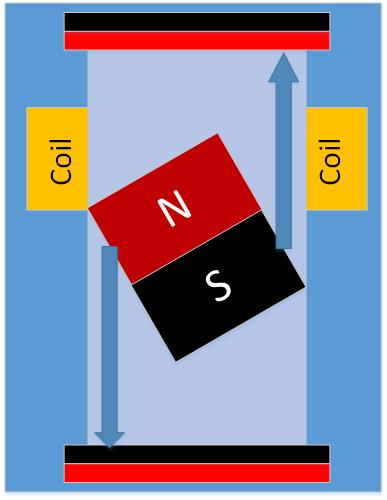
\includegraphics[height=6cm]{images/own_dwg/generator_torgue}
\end{center}
\caption{Angle in magnet causes torque which results in increased friction}.
\label{fig:lg_torgue}
\end{figure}



\subsubsection{Analytical model of the electromagnetical vibration harvester}
A common starting point for analysis of linear generator is to model the mechanical domain as Mass-Spring-Damper system depicted in Figure \ref{MSD}. A mass "floats" in the system, a spring balances the mass towards the centre and a damper represents frictional forces opposing any movement of the mass. 

\begin{figure}[htb]
\begin{center}
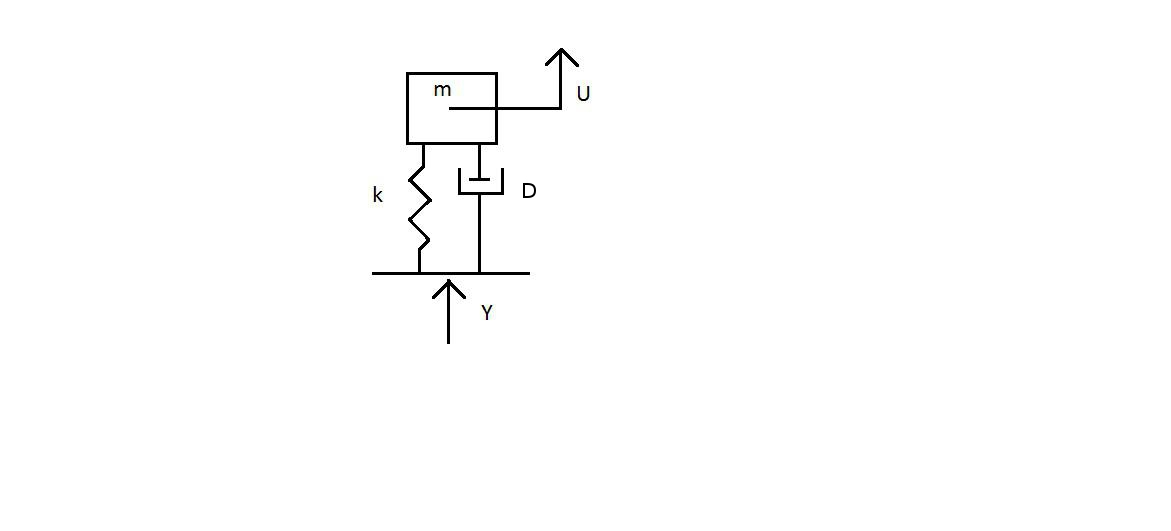
\includegraphics[height=6cm]{images/own_dwg/MSD.jpg}
\end{center}
\caption{\label{MSD} Mass-spring-damper system.}
\end{figure}

Mathematical representation of this system is given in Equation \eqref{eq:MSD_basic}. Input Y is the force applied to the base of system, output U is the position of mass block relative to "zero". Zero is usually set to the point where the mass settles when no input, including gravity, is applied to the system. Parameters m, D, and k are mass, damping constant and spring constant of system, respectively. Input-output-equation in time domain can be written as: 

\begin{equation}\label{eq:MSD_basic}
  m \cdot \ddot{U}(t) + D \cdot \dot{U}(t) + k \cdot U(t) = Y(t). 
\end{equation}
As the force $ Y(t) $ is defined as $ Y(t) = m \cdot a(t) $, and the acceleration $ a(t)$ can be considered constant regardless of any reasonable mass $ m $ of system, equation \eqref{eq:MSD_basic} can be written as:

\begin{equation}\label{eq:MSD_acceleration}
 \ddot{U}(t) + \frac{D \cdot \dot{U}(t)}{m} + \frac{k \cdot U(t)}{m} = a(t). 
\end{equation}
This form is more convenient for analysis, as the acceleration measurements from previous research are available and they represent real-world values. Mass $m$ can be considered constant, as the system does not exchange matter with surrounding environment. As magnetic suspension was selected, the parameter $k$ cannot be considered as a constant, but rather a function of mass position $k(U)$. Centripetal force can be considered as a constant DC-component of function $Y(t)$, and is not included in analysis of function $k(U)$. According to D. Amrani \cite{Amrani2015} force between two magnets can be approximated as

\begin{equation}\label{eq:magnetic_force}
  F(x) = \frac{3 \mu_0 m_1 m_2}{2 \pi} \cdot \frac{1}{x^4},
\end{equation}
where $F(x)$ is force as a function of distance $x$ between magnets, $\mu_0$ is the permeability of vacuum, $ m_1 $ and $ m_2 $ are magnetic dipole moments of magnets under examination. This equation is only valid when $x >> h$, where $h$ is thickness of the magnet. As two magnets are used to suspend the rotor magnet, total force acting on mass becomes 

\begin{equation}\label{eq:magnetic_force_middle}
  F(x) = \frac{3 \mu_0 m_r m_l}{2 \pi} \cdot \frac{1}{(x_0+x)^4} - \frac{3 \mu_0 m_r m_u}{2 \pi} \cdot \frac{1}{(x_0-x)^4},
\end{equation}
where $m_l, m_u, m_r$ are magnetic dipole moments of lower suspending magnet, upper suspending magnet, and rotor magnet. $x_0$ is the distance to middle point of generator and $x$ is the displacement of rotor magnet from aforementioned middle point, positive direction being upwards. Figure \ref{fig:lg} shows the system.

\begin{figure}[htb]
\begin{center}
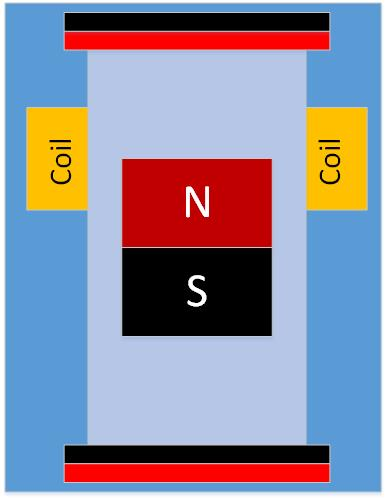
\includegraphics[height=6cm]{images/own_dwg/generator}
\end{center}
\caption{Linear generator with rotor magnet balanced by endstop magnets}.
\label{fig:lg}
\end{figure}

However, the Equation \eqref{eq:magnetic_force_middle} is very inaccurate for magnets which have the diameter larger than the thickness, and the problems are compounded when distance between magnets is small. Therefore final design was optimised using Finite Element Analysis (FEA) for determining $k(U)$. 

Damping parameter $D$ is likewise a function of electromagnetic force acting on the magnet, friction between the magnet and the stator and pneumatic damping caused by compression of air in the generator. Tornincasa et al. \cite{Tornincasa2012} divided this damping parameter into three distinct terms to account for these different physical phenomena in damping. Let us call them $D_{emf}, D_{friction},$ and $D_{air}$, respectively. $D_{emf}$ represents power extracted from the system into electrical current, it can be written as:

\begin{equation}\label{eq:d_emd}
  D_{emf} = BIl \cdot sin(\phi),
\end{equation}
where $B$ is magnetic field affecting coil (presumed constant), $I$ is current through wire depending on load and generator properties, $l$ is total length of wire in coil and $\phi$ is angle between coil and magnetic field, presumed to be 90 \degree. Assuming the load impedance is the complex conjugate of coil impedance for maximum power harvesting, we can substitute the $I$ with equations \eqref{eq:emf} and \eqref{eq:gen_simple_current}, which results in: 

\begin{equation}
  D_{emf} = B \frac{\varepsilon}{2 \cdot Re(Z_{generator})} l sin(90 \degree),
\end{equation}
where $Z_{generator}$ is the impedance of generator. As the load impedance is complex conjugate of generator impedance, their series connection has only real (purely resistive) component. This assumption fails on real-world application with non-linear rectification and DC/DC conversion, but it can be used as a basis for analytical examination of the generator. As $\varepsilon$ can be substituted with \eqref{eq:emf}, we obtain:

\begin{equation}\label{eq:d_emf_with_epsilon}
  D_{emf} = B \frac{-N \frac{d \Phi_{B}}{d t}}{2 \cdot Re(Z_{generator})} l \cdot sin(90 \degree),
\end{equation}
The relationship between $N \Phi_{B}$ and $Re(Z_{generator})$ can be further studied by writing: 

\begin{equation}\label{eq:phiB_substitution}
  \Phi_{B} = \iint_{\Sigma (t)} B(r, t) \,dA,
\end{equation}
where $ \iint_{\Sigma (t)} $ signifies possibility of the loop area changing over time and $\,dA$ is an element of the surface area. If we assume the coil to be a perfect tightly wound circle which does not deform over time, we can write the relationship between number of turns in the coil, area of the coil, and resistance of the coil as:

\begin{equation}\label{eq:nA_R}
  R = N 2\pi \r_{coil} \frac{\rho_{wire}}{A_{wire}},
\end{equation}
where $\r_{coil}$ is the average radius of coil, $\rho_{wire}$ is the resistivity of the wire and $A_{wire}$ is the cross section of the wire. Substituting Equations \eqref{eq:nA_R} and \eqref{eq:phiB_substitution} into Equation \eqref{eq:d_emf_with_epsilon} we finally obtain expression for $D_{emf}$ which accounts for the design parameters affecting it:
\begin{equation}\label{eq:d_emf_complete}
  D_{emf} = B \frac{-N \frac{d [\iint B(r, t) \,dA]}{d t}}{2 \cdot N 2\pi \r_{coil} \frac{\rho_{wire}}{A_{wire}}} l sin(90 \degree).
\end{equation}

A few observations can be made from this equation: first, the magnetic field strength $B$ and its derivative in respect to time increase the $D_{emf}$ which signifies the electrically extracted useful power. Therefore it makes sense to use as strong magnets as possible as long as other parameters aren't adversely affected, in effect by using magnets made of strongly magnetic alloy. Second, both the number of turns $N$ and the loop area $A$ are in nominator and denominator, which means they should be optimised to find the best applicable values. Third, resistivity of wire limits the power that can be extracted, so intuition would lead to minimising the wire resistance. In practise the wire resistivity can be decreased by increasing the wire diameter, which in turn leads to lower number of turns in same the volume and mass of the coil. Therefore, also wire diameter and material should be optimised to find desirable compromise in the generator design. 

Next we examine $D_{friction}$ in detail. Friction is modelled as Coulomb friction:
\begin{equation}\label{eq:Coulomb_friction}
  F_s = \mu_sN,
  F_k = \mu_kN,
\end{equation}
where $F_s $ and $ F_k $ are static and kinetic friction forces opposing movement, $\mu_s$ and $\mu_k$ are friction coefficients in static and kinetic situations and $N$ is normal force along X- or Y- axis. Normal forces are estimated by using the existing acceleration data and calculated mass of magnet. Coefficients of friction are looked up from the supplier of stator material. Transfer between static and kinetic models is assumed to be a step, if velocity of magnet is 0 along Z-axis, $\mu_s$ is used, $\mu_k$ otherwise.

Finally, there is pneumatic damping of the system, $D_{air}$. In a closed tube, the central magnet can be thought of as a piston dividing the generator into two chambers. If there is an insignificant airflow between chambers, any force caused by pressure deltas between chambers act as a spring. However, some airflow is to be expected due to the clearance between the magnet and the stator. Tornincasa et al. \cite{Tornincasa2012} modelled this effect by adding a virtual centrepoint for the pneumatic spring. This centre moves through a virtual damper which models the airflow between the chambers. End result is that the pneumatic spring takes some energy from movement, and the energy stored into pneumatic spring is dissipated as the centre moves until potential energy stored in the spring is zero. 

The force from pressure differential is:

\begin{equation}
  F_{\delta p} = \frac{\pi d^2}{4}(p_{lower}-p_{upper}),
\end{equation}
where $d$ is diameter of magnet and $p_{lower}-p_{upper}$ are pressures in chambers. Pressures can be estimated from ideal gas law:

\begin{equation}
  pV = NRT
\end{equation}
where $p$ is pressure, $V$ is volume, $N$ is amount, $R$ is ideal gas constant and $T$ is temperature. Temperature is assumed to be constant. Initial pressure is assumed to be same as tyre pressure and magnet is assumed to be exactly in midpoint at start. Change of volume can be calculated from change of height caused by movement of the magnet. 

Mass flow between sections can be estimated with equation given by Fox et al. \cite{Fox2008}:

\begin{equation}
  \dot{m}_{1 \rightarrow 2} = \frac{\rho \pi d {\delta_r}^3}{12\mu h}(p_1-p_2),
\end{equation}
where $\rho$ is air density, $\delta_r$ is radial clearance, $\mu$ is dynamic viscosity and $h$ is the height of magnet. \cite{Tornincasa2012}

There is also frictional dissipative force as the air passes along the edges of the cylinder. This frictional force has magnitude of \cite{Medhat2008}: 

\begin{equation}
  F = \mu \cdot \rho \cdot \frac{\pi d h \dot{z}}{\delta}  
\end{equation}

Analytical expressions for the equations governing the mechanical movement of magnet inside generator have now been identified. Some of the non-linear functions are hard to solve analytically, therefore experimental and FEA methods are used for creating approximations for these functions. The analytical effect of these parameters is summarised in Table \ref{parameters_of_lg}.

\begin{table}[htb]
\caption{\label{parameters_of_lg} Effect of the parameters of the generator.}
\begin{center}
\fbox{
\begin{tabular}{l l l}
\textbf{Parameter}          & \textbf{Increasing} 		& \textbf{Decreasing}	\\ \hline
\(\displaystyle N_{turns} \)& Higher voltage		& Smaller size, less wiring resistance 		\\ \hline
\(\displaystyle N_{pole} \) & Increased frequency		& Decreased frequency	\\ \hline
\(\displaystyle l_{pole} \) & More space for wiring 	& Higher voltage, smaller size	\\ \hline
\(\displaystyle A_{loop} \) & More power			& Smaller length of wiring 	\\ \hline
B                           & Increased power 	        & Smaller magnets 		\\ \hline
\(\displaystyle r_{wire}\)  & Decreased wiring resistance 	& More turns in same space 	\\ \hline
\(\displaystyle \delta_{r} \) & Stronger side walls		& Increased efficiency 
\end{tabular}
}
\end{center}
\end{table}

This section has given analytical expressions on forces acting on the magnet. With the expressions known, next section presents simulation and experimental methods for evaluating the effects of these expressions.

\subsubsection{Experimental and FEA modelling of the electromagnetic harvester}
Some parameters of the harvester are difficult to solve analytically. These parameters are estimated using experimental and Finite Element Analysis (FEA) methods. First one of these difficult interactions is the magnetic force between rotor magnet and balancing magnets. A magnetics FEA software FEMM \cite{Meeker2013} was used to create an axisymmetric model of magnets in the generator. Figure \ref{femm_forces} shows the used model. This model has two opposing magnets made of N40-neodymium alloy configured to repel an identical rotor magnet. The magnets have a height of 2.5 mm and diameter of 11 mm, walls of generator are modelled as air. The generator has total height of 25 mm, leaving the rotor magnet 17.5 mm room for movement inside the generator.

Weighted stress tensor integration over rotor magnet volume as implemented by FEMM was used to determine FEA value for the net magnetic force acting on the rotor magnet. A LUA script was used to move the rotor magnet from the bottom of the generator to the top in 0.1 mm increments and values obtained from the analysis were exported as CSV data for plotting in a spreadsheet software. Figure \ref{femm_forces} shows the force on the magnet, positive force meaning force towards the upper magnet and zero height being at in the middle of the cylinder. The centrifugal force acting on magnet was also calculated at various speeds for reference, assuming weight of the magnet is 1.67 g and radius to the bottom of generator is 275 mm.

\begin{figure}[htb]
  \begin{center}
  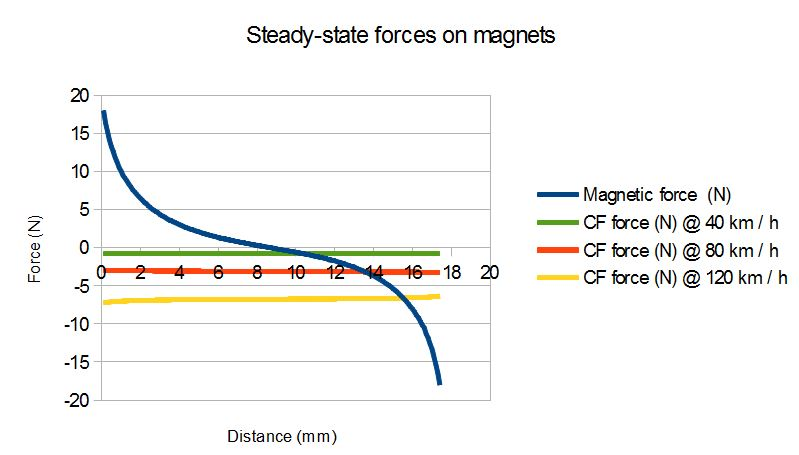
\includegraphics[width=\columnwidth]{images/own_dwg/femm_fvsd_dualmagnet.jpg}
  \end{center}
  \caption{\label{femm_forces} Steady-state forces acting on a magnet. The magnetic force will counteract centrifugal force at 2 mm, 5 mm and 7 mm displacement from center for speeds of 40, 80 and 120 km / h respectively.}
\end{figure}

It can be seen that net force on rotor magnet is dominated by the magnetic forces at lower speeds from points where magnetic force graph intersects centrifugal force line. Centrifugal force on magnet becomes significant at higher speeds. The rotor magnet can impact the bottom assuming 20 mm displacement as estimated in Figure \ref{fig:deformation} in Section \ref{sect:tyre_environment}, therefore rubber layer to act as a bumper may be required on stator magnets. Second use for this FEA analysis was to create a look-up table for flux linkage into the coils of the generator. The methodology was similar to determining the forces affecting the rotor magnet: a LUA script was ran to sweep the possible magnet positions, and the look-up table of flux linkage into coils was created. For the purposes of analysis, difference of flux linkage was calculated between each point. The change of flux linkage is a very important parameter, as the power generated is proportional to $\frac{d \Phi_{B}}{d t}$. 

\begin{figure}[htb]
\begin{center}
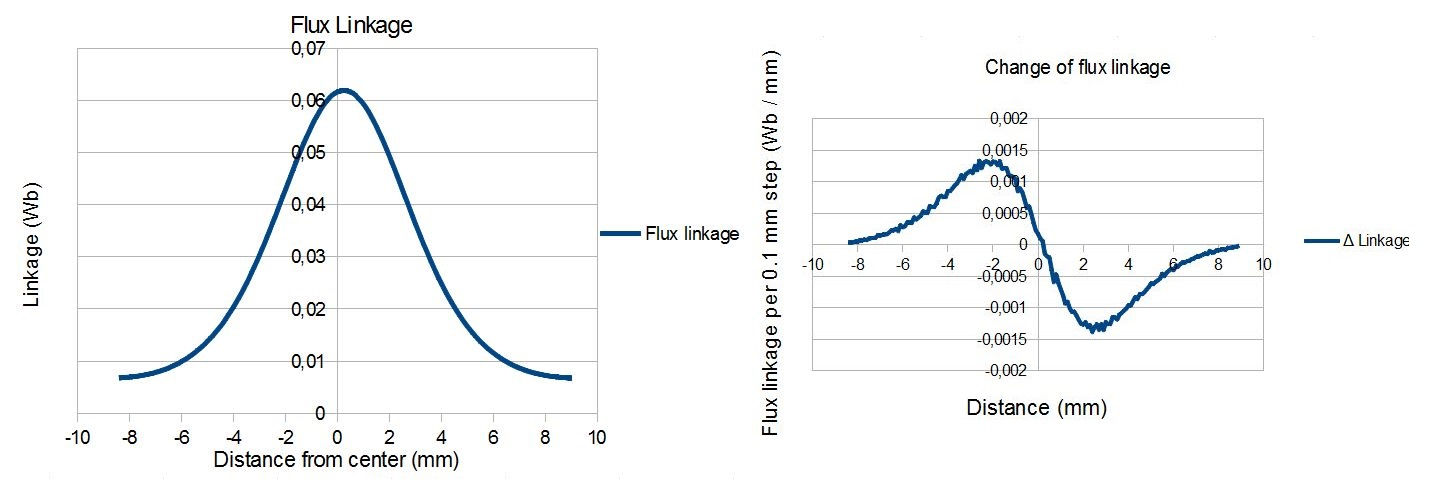
\includegraphics[width=\columnwidth]{images/own_dwg/femm_flux_dualmagnet.jpg}
\end{center}
\caption{\label{fig:femm_linkage} Flux linkage and rate of change in 0.1 mm steps in generator. Derivative of flux linkage in respect to position is largest near 2 - 3 mm displacement from the centre of the coil.}
\end{figure}

Based on these results, a magnet moving at the speed of 0.1 mm / s would induce voltage up to 1.5 mV  in each winding of the coil.

\begin{comment}

A prototype generator was built to test the concept feasibility and identify any practical issues in the generator construction. Generator was machined out of 21mm diameter nylon tubing with 12 mm inner diameter. A groove was machined on the outer diameter to hold the coiling in place. Inner diameter of the groove was 14 mm and height 3 mm. A 0.1 mm diameter wire was used to build the coil. To determine the number of turns in coil, coil resistance was measured to determine the length of wire and number of turn was calculated using known length of loop turn and total length of wire. Coil resistance was 42 ohms as the resistance of wire is approximately 2.2 ohms / meter the total length is approximately 19 meters. As one loop has length of 44 mm, coil had roughly 400 turns. 

The prototype was connected on a  Brüel \& Kjær shaker type 4905 and driven using  Brüel \& Kjær power amplifier type 2707. Input signal was generated using NI-USB6218 DAQ and output was measured directly from leads of the generator. Vertical displacement of generator was limited to $7.5 mm$. Output signal was a sine wave with amplitude of $\pm$ 5 volts, which was amplified by gain of 8 above frequencies of 30 Hz. At lower frequencies the gain was limited to stay within allowed displacement. Measured graphs are shown in figure \ref{fiq:lg_proto_results}.

\begin{figure}[h]
\begin{center}
  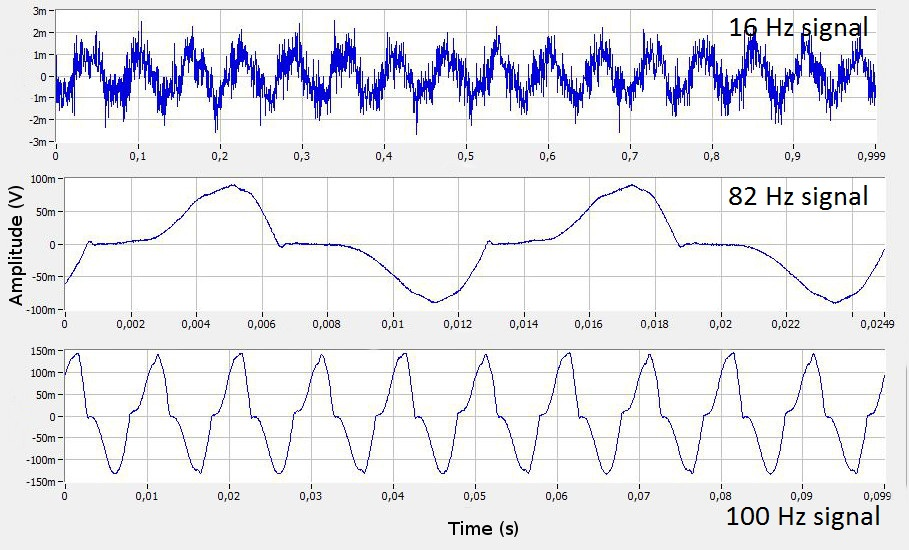
\includegraphics[height=8cm]{images/own_measurement/lg_proto.jpg}
  \end{center}
  \caption{\label{fiq:lg_proto_results} Measured open-loop voltage outputs at various frequencies}
\end{figure}

At low frequencies the magnets do not overcome friction and only measurement noise is present in signal. In addition to white noise in measurement there is a sine wave with amplitude of hew millivolts which correlates with the excitation signal. The measurement noise is insignificant when compared to signal generated my moving magnet. 

At low frequencies the magnet cannot overcome the friction and only noise is present in measurement. Around 82 Hz the magnet could move inside shaft, producing peaks with roughly 100 $mV$ peaks. The magnet stops in between of the peaks which is seen as valleys of no voltage being produced. 

Peak voltages of roughly 150 mV were achieved at 100 Hz. The magnet is in almost constant motion, a brief stop can be seen when the magnet changes direction. 

While 150 mV is notably less than the few volts predicted by Simulink model, the basic operation principles was validated by quick experiment. The difference in output voltage is probably due to imprecise construction in prototype harvester. As the concept was proven, the design of generator was finalised. Next section details the exact construction of final electromagnetic generator. 

\subsubsection{Mechanical design of electromagnetic harvester}\label{sect:emh_design}
Few practical issues became evident during construction of prototype generator. Machining grooves to plastic tubes caused warping to tube, which prevented magnet from moving inside coils. Shallow grooves would not keep the coils in place, as wires being loose would fall off the groove. The tube did not offer any reasonable mount point for a printed circuit board. 

Issues with grooves were solved by selecting a tube with minimal wall thickness and using separators to contain the coil. A separate housing was designed to hold the tube and to offer mounting points for the circuit board. 

A layered design was made for the harvester. On the bottom is a solid square with 35 * 35 mm sides and holes for screws on corners. Next layer has a hole for the bottom magnet, third layer has hole for the tube. Tube has a spacer in middle to hold the coil below midpoint. Top half of harvester is symmetrical to bottom. 

\end{comment}

\subsection{Piezoelectric harvester design}
\subsubsection{Basics of the piezoelectric energy harvesting }
This section details experimental identification of properties of the piezoelectric element used in the harvester. A testbed with an impactor providing excitation was used to generate experimental values for power output and voltage at various operating conditions for the piezo element.

Thunder\textsuperscript{(TM)} piezos have been used in previous studies of piezoelectric harvesting and they have produced promising results \cite{Manla2009}, so they were selected as the piezoelectric element for this thesis.

Series of tests were ran to determine the characteristics of piezoelectric power generation under impacts. Mossi et al. \cite{Mossi} have produced a recommended test process for Thunder piezoelectric actuators shown in Figure \ref{fiq:thunder_eval}.

\begin{figure}[htb]
  \begin{center}
  \includegraphics[height=6cm]{images/cited/mossi}
  \end{center}
  \caption{Recommended evaluation platform for Thunder piezos \cite{Mossi}.}
  \label{fiq:thunder_eval}
\end{figure}

This setup was replicated using a solenoid actuator as an impact force generator, a precision scale as load cell to measure the impact force and an oscilloscope to view the output waveforms. An eraser was cut to shape to act as preload bellow to spread the impact over larger surface area of piezoelement. Displacement was not measured. The test setup is shown in Figure \ref{fiq:piezo_impact}. An electronics prototyping platform, "breadboard", was used to house test the electronics including a resistive ladder and an Arduino to trigger the solenoid at adjustable duty cycles. Load force was controlled by setting the stroke length of the solenoid shaft and fine tuned by adjusting the voltage over the solenoid. 

\begin{figure}[htb]
  \begin{center}
  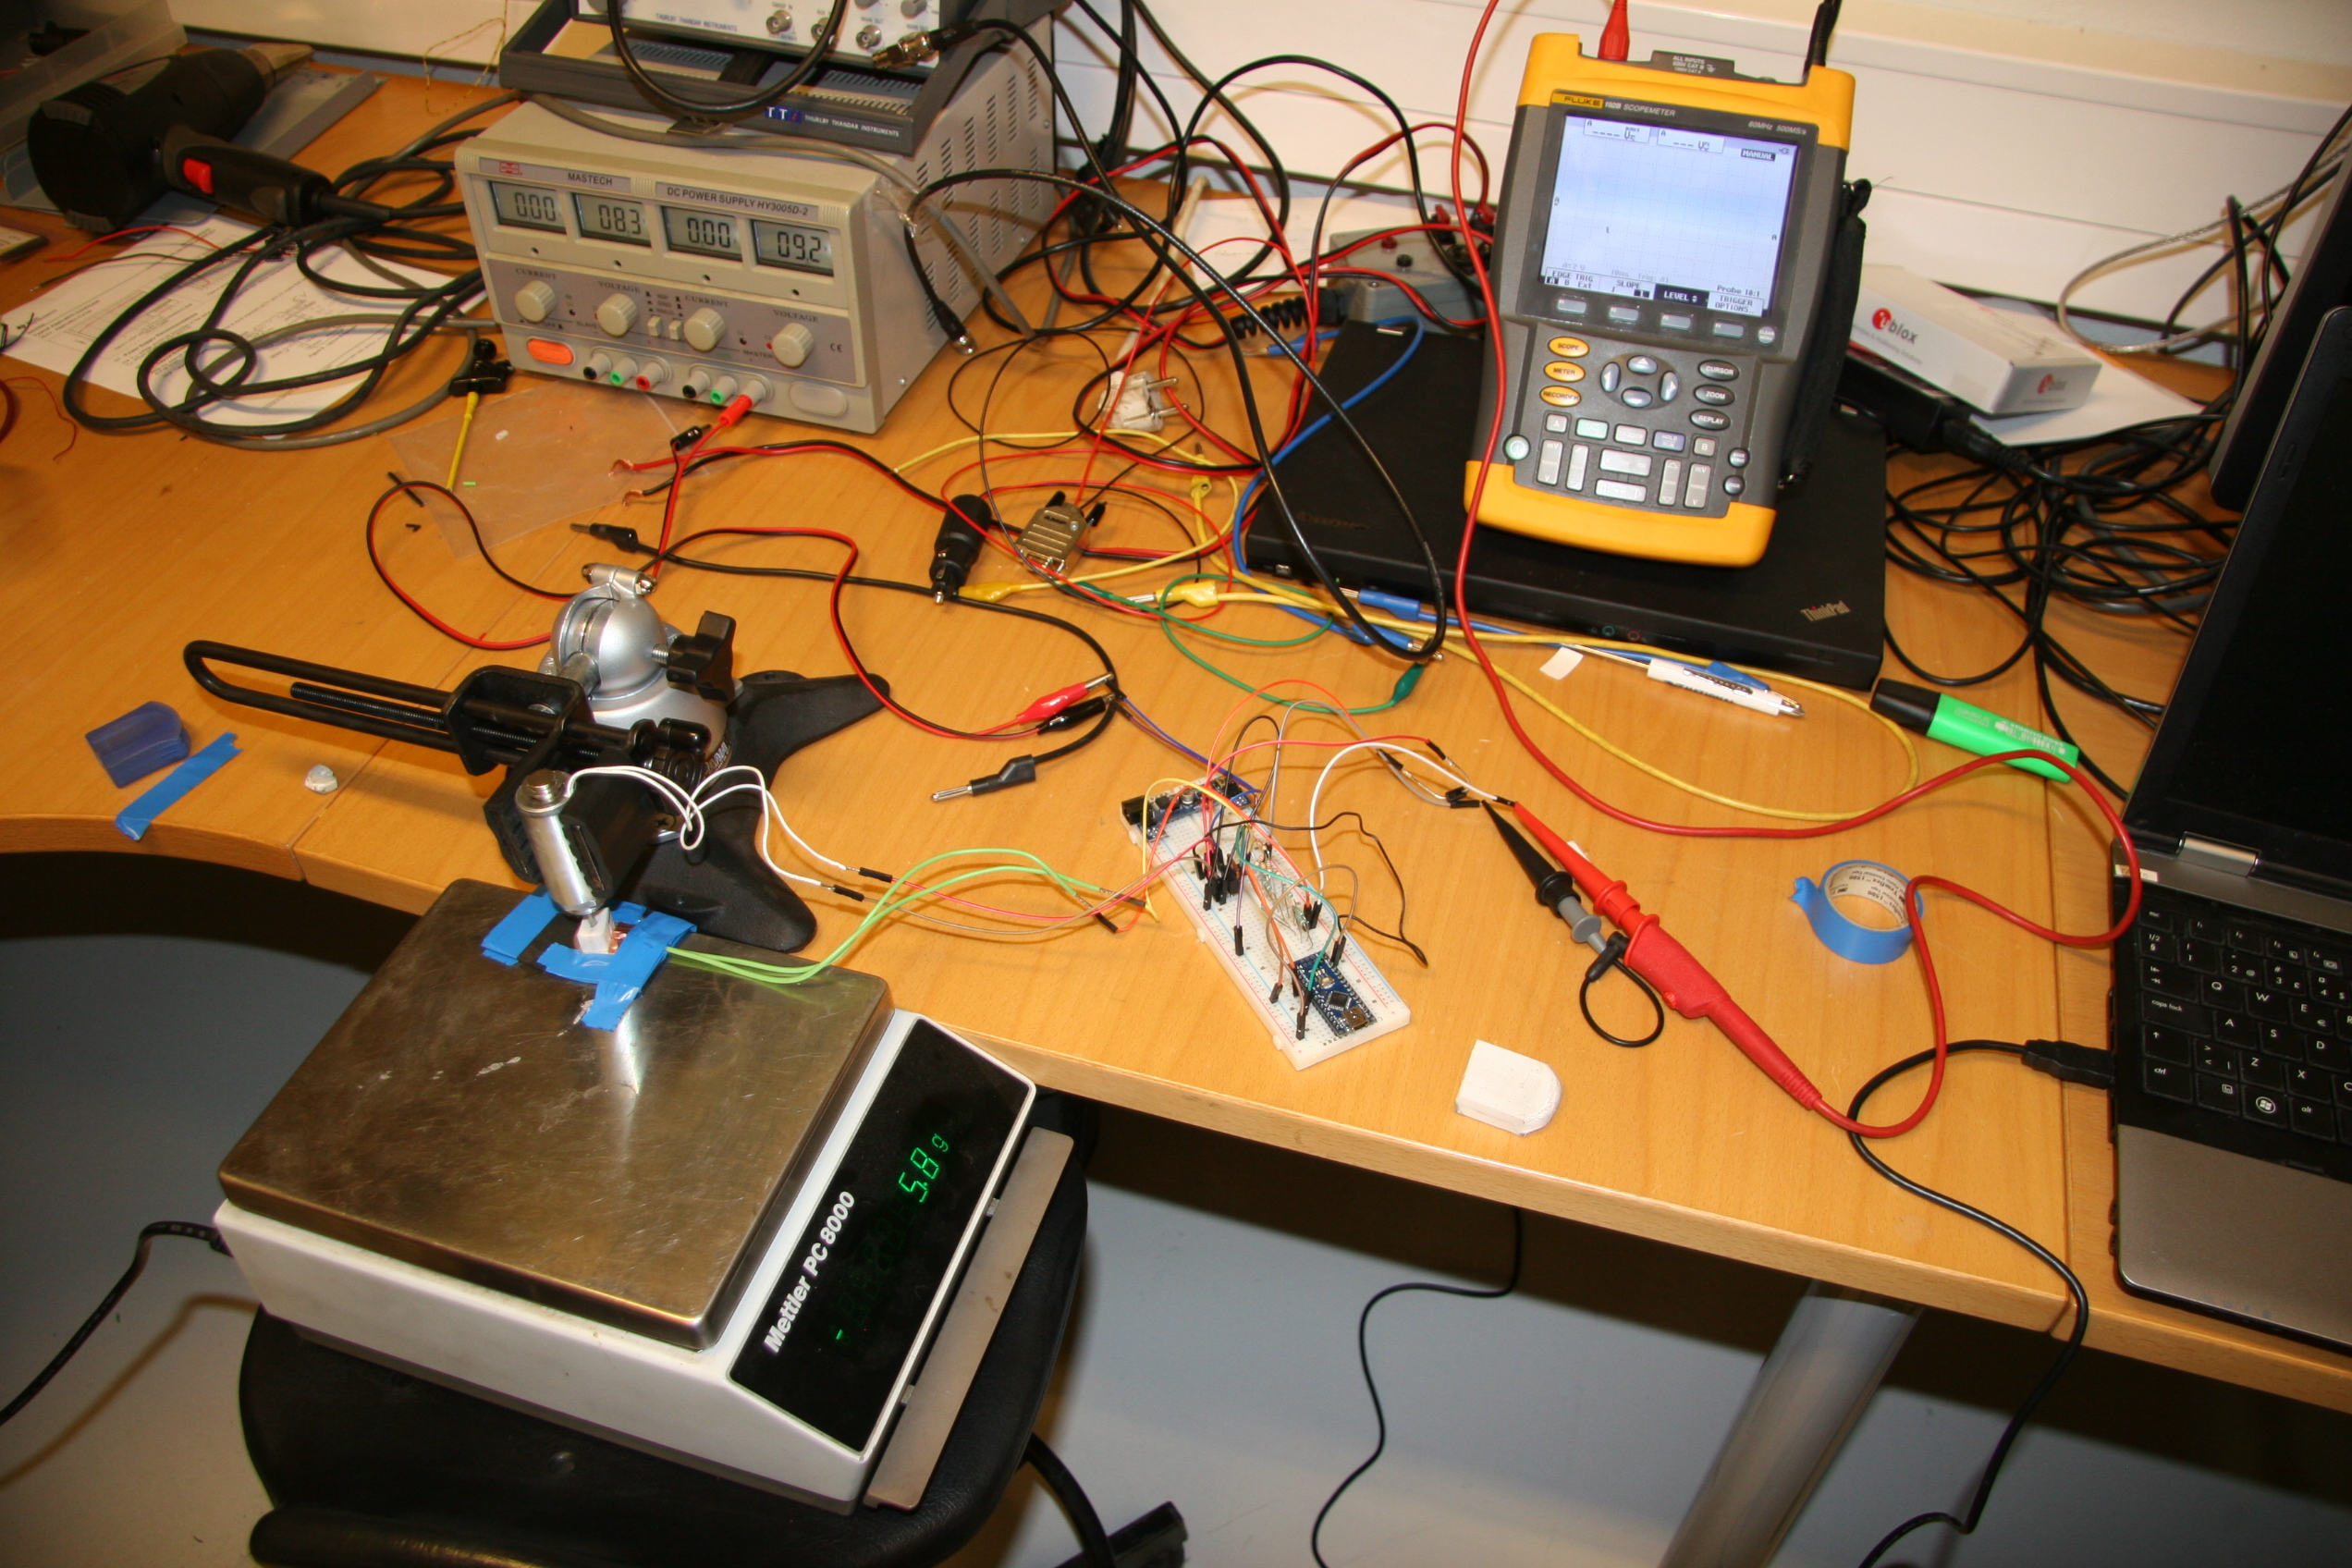
\includegraphics[height=6cm]{images/own_pic/piezo_test}
  \end{center}
  \caption{Test platform for piezo characteristics.}
  \label{fiq:piezo_impact}
\end{figure}

The measurement results are shown in Figure \ref{fiq:piezo_measurement_chart}. Output voltage scales with square of impact force, which is sensible as the work done can be expressed as $W = F \cdot d$, where $W$ is work, $F$ is force and $d$ is a distance the force acts on an object. As the displacement of the piezoelement grows with the applied force, total work and therefore energy grows with the both terms. 

\begin{figure}[htb]
  \begin{center}
  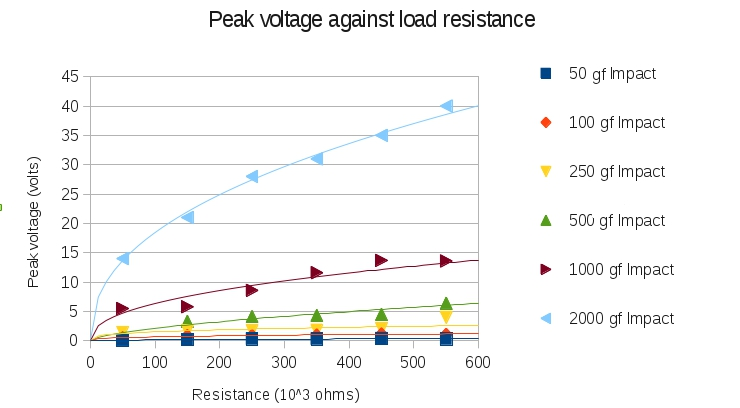
\includegraphics[height=6cm]{images/own_measurement/piezo_measurements}
  \end{center}
  \caption{Measured output voltage at different loads and impact forces.}
  \label{fiq:piezo_measurement_chart}
\end{figure}

Peak voltage grows with the load resistance. This is in agreement with both the voltage source and the current source models, as the capacitor starts to discharge through the load resistance instantly when a voltage is applied over it. The relationship between voltage and load resistance seems to be logarithmic, which would be in an agreement with the logarithmic discharge curve of the capacitor-resistor system. Peak voltages were read out from a digital display and they can be considered reasonably accurate.

The time constants for a voltage halving were graphically measured from oscilloscope waveforms, and this data was used to calculate the capacitance of TH-5C. These measurements are a lot less accurate, as readouts from an oscilloscope screen have resolution of approximately half of the line division, making the accuracy of measurements at $\pm 2.5 ms$. These results are shown in Figure \ref{fig:piezo_time_capacitance}

\begin{figure}[htb]
  \begin{center}
  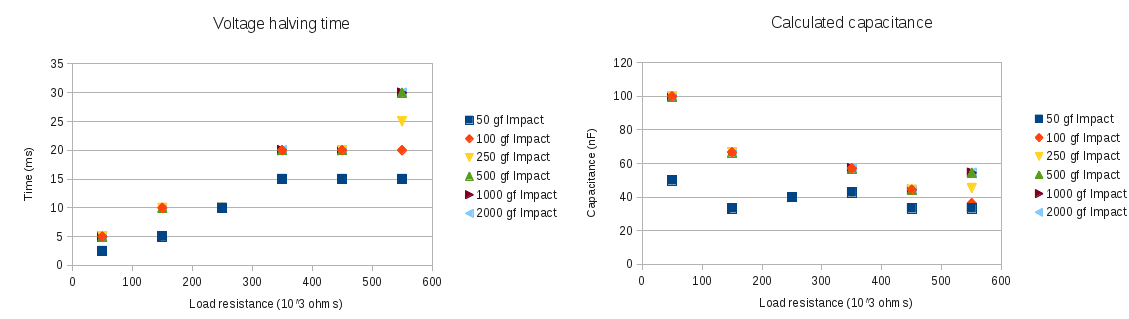
\includegraphics[width=\columnwidth]{images/own_measurement/piezo_capacitance}
  \end{center}
  \caption{Measured half-time of system and the calculated capacitance of the piezoelement.}
  \label{fig:piezo_time_capacitance}
\end{figure}

The half-time data can be used to calculate the capacitance of the piezoelement using the RC-time constant of circuit:

\begin{equation}
  C=\frac{t}{-ln(\frac{1}{2})R} 
\end{equation}

Datasheet of TH-5C provides a value of 39 nF as the capacitance, while these calculated values are notably higher and rise with the loading of the piezoelement. Most likely explanation of this observation is the mechanical response time of system: the solenoid plunger will take some milliseconds to reach new force equilibrium, and this effect becomes more pronounced at smaller time constants of the RC-system. Using the known voltage and capacitance energy and peak power in impact can be determined:
 
\begin{equation}
   E = \frac{1}{2}V^2C
\end{equation}

\begin{equation}
   P_{peak} = \frac{V^2}{R}
\end{equation}
 
The results of calculations are shown in Figure \ref{fig:piezo_power_energy}. As these calculations are based on inaccurately measured time, they should not be used as reference for any further calculations. However, trends can be seen in these values. 
 
 Interestingly the peak work done by the piezoelement to the resistor seems to be almost constant on all load levels. This is probably a consequence of the logarithmic voltage-load relationship described earlier in this section. There is a possibly significant result based on these findings: total energy obtainable from harvester grows with the load resistance. However, this is applicable only for a resistive load under impact-based energy generation.
 
 \begin{figure}[htb]
  \begin{center}
  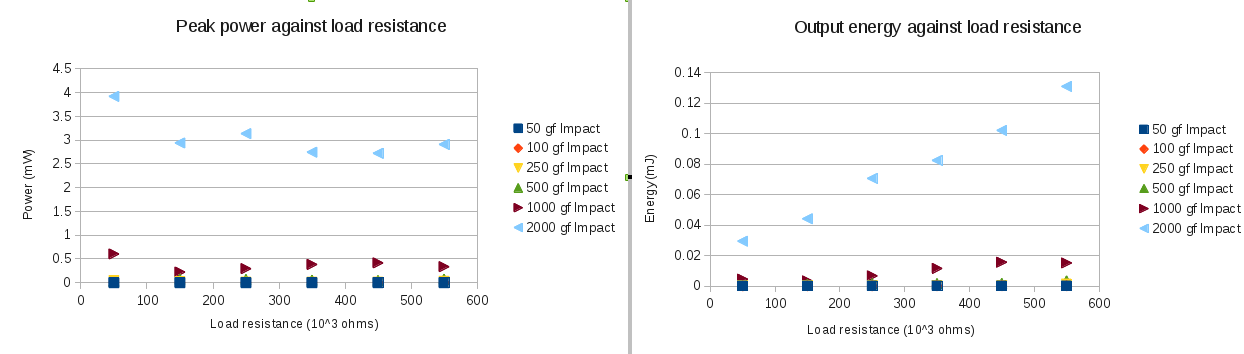
\includegraphics[width=\columnwidth]{images/own_measurement/piezo_power}
  \end{center}
  \caption{Calculated piezo power and energy output. Power output is almost constant at all loads, but energy generated during impact grows with load resistance.}
  \label{fig:piezo_power_energy}
\end{figure}

Based on these results, an electrical equivalent model of the circuit was designed. The model is shown in Figure \ref{fig:piezo_ltspice_equivalent}. Model has two parallel current sources, one to simulate impact of the plunger on the piezoelement and other to simulate the release of the impact. Capacitance in parallel is set to 39 nF as given in the datasheet, load resistance is parametricised to step through the experimental values.

Model was tuned by first calculating the total current transfer to reach the open circuit voltage over capacitor. Then maximum current of current sources was matched to the peak voltage over highest load.
The simulated data is plotted Figure \ref{fiq:piezo_simulation_experimental}.

 \begin{figure}[htb]
  \begin{center}
  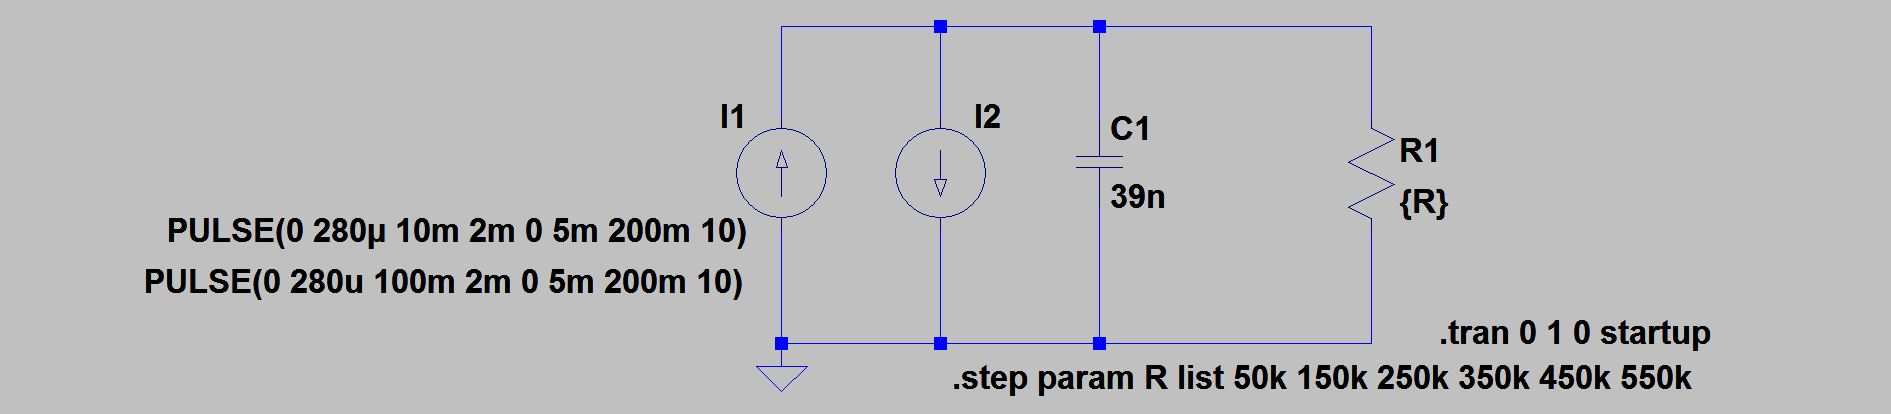
\includegraphics[height=6cm]{images/own_dwg/ltspice_piezo}
  \end{center}
  \caption{Equivalent model of piezo in LTSpice simulator.}
  \label{fig:piezo_ltspice_equivalent}
\end{figure}

 \begin{figure}[htb]
  \begin{center}
  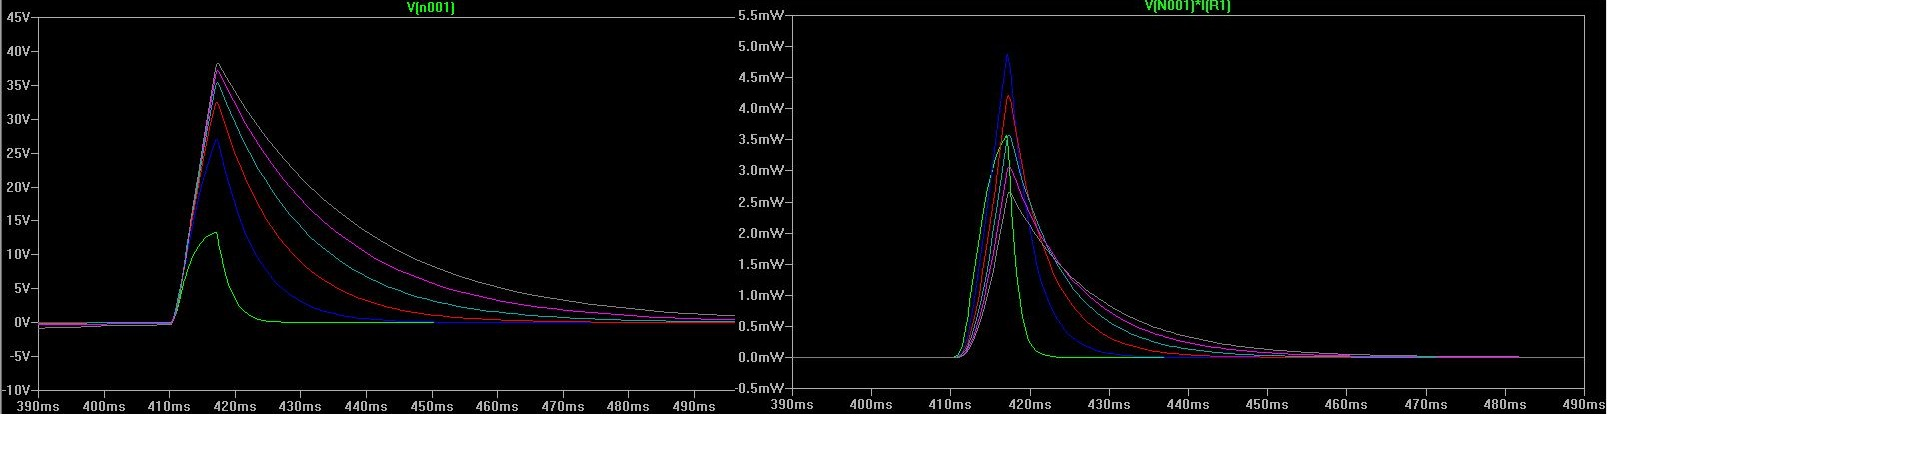
\includegraphics[height=8cm]{images/own_dwg/ltspice_piezo_simulation}
  \end{center}
  \caption{Simulated piezoelement output voltage and power waveforms. Loads are stepped through list to match experimental values at 2000 gf impact force. Black: 50k; Blue: 150k; Red: 250k; Green: 350k; Pink: 450k; Gray: 550k}
  \label{fiq:piezo_simulation_experimental}
\end{figure}

The experimental and simulated data are not in an agreement. While maximum and minimum load voltage and power are close to estimated values, this is by design as the model is tuned to these measurements. Problems occur in interpolating the results, as output voltages are notably higher than measured values. This provides a result which sets the maximum power load near the value which provides output voltage of half of the open loop voltage. However this result is valid only for resistive load, and therefore rectified power output might have different characteristics. 

\subsection{Electronic design} \label{sect:electronic_design}
\subsubsection{Simulation of the circuit}
As the focus of work is on energy harvesting, only analog sections related to energy harvesting are simulated. This section details the simulation model used to validate the design of circuitry.

The analog sections of circuit were simulated using LTSpice IV \cite{ltspice}. Digital loads are simulated as current sinks. Battery was modelled as a voltage source with high-value capacitor and low-value resistor in series. Piezoelectric harvesting was modelled both as high-voltage source with capacitor in series, and as a current source with capacitor in parallel. Electromagnetic harvesting was modelled as low-impedance low-voltage source. 

LTC3331 presents an interesting opportunity for maximum power point tracking (MPPT). While the impedance of individual components cannot be tuned in real-time, the microcontroller can determine the rotation frequency of the tyre from the accelerometer readings and determine the maximum power point. LTC3331 can adjust the target voltage for the energy storage buffer capacitor, which enables MPPT-control of system.

The simulation model is shown in Figure \ref{fig:ltspice_sim}. Connections were adjusted as needed to generate simulation data for different purposes, such as measuring energy efficiency, transient response, MPPT etc.

\begin{figure}[htb]
\begin{center}
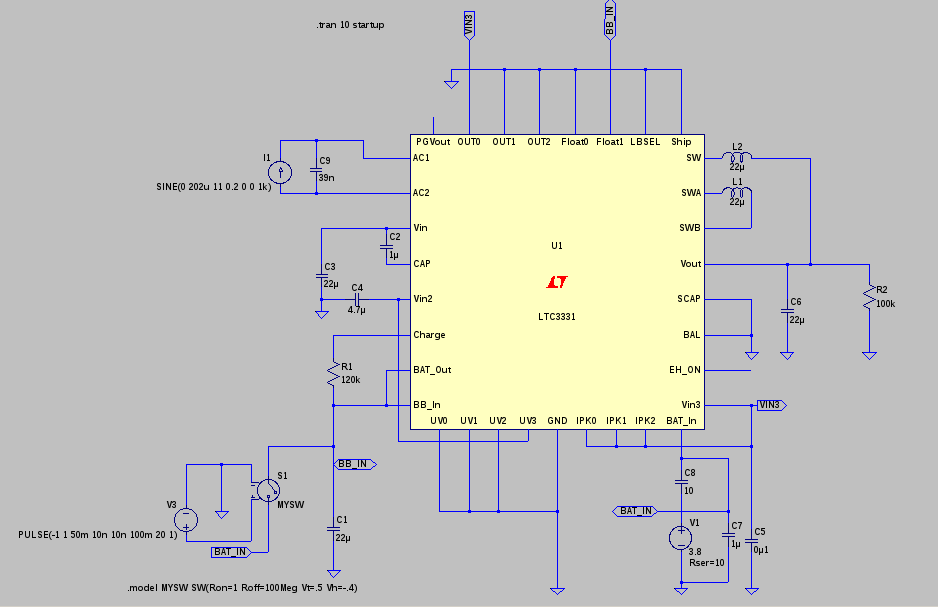
\includegraphics[height=12cm]{images/own_dwg/ltspice_ltc3331.jpg}
\end{center}
\caption{\label{fig:ltspice_sim} LTSpice \cite{ltspice} simulation of electrical circuit}
\end{figure}

The simulation model was used to validate the basic operation of the circuit, circuit operates as the datasheet specified. As the basic operation of circuit has been validated, next step was to design the detailed schematic for the circuit. The next section details schematic design of the circuit, starting from top-level diagram and connections between blocks, followed by detailed design of each subblock. 

\subsubsection{Schematic design}
The schematic is a logical representation of the components and how they connect to each other. The schematic is designed in accordance with the datasheets, reference designs and application notes of the main circuit components. This section details the schematic diagram of the circuit.

As the design operates in a high-vibration environment with wide temperature variations, special care was used to select components which have well-defined temperature and mechanical characteristics. 

Since the circuit is a low-power design, careful attention was paid to parasitic properties and non-ideal behaviour of components. For example electrolytic capacitor can have leakage current of several microamperes \cite{Both2001}, which is in the same order of magnitude as the targeted sleep current consumption of system. Likewise any signalling current was kept at minimum. 

Another important point of view is the modularity and testability of the circuit. All critical lines have provision for testing and debugging for development and verification of the circuit functionality. Figure \ref{fig:circuit_blocklevel} shows the interconnections in system, drawn in KiCAD \cite{KiCAD}.  The power supply can be cut off to separate sections of circuit for current measurement as needed. This has additional benefit of leaving places for power supply filtering components in case some section of circuit emits electrical noise through power supply lines.

\begin{figure}[htb]
    \centering
    \def\svgwidth{\columnwidth}
    \input{images/own_dwg/circuit/radio.pdf_tex}
    \caption{\label{fig:circuit_blocklevel} System level design of electronics. Block "power management" contains the energy storage and management functions, "Control" has microcontroller which handles MPPT. Sensor block communicates with with control block and control can preprocess the data before sending it over to radio link. All the subblocks are presented in detail in this section. Top-level diagram shows the external connections to system and test points between the sections. Experimental section of the work implements only Power Management functions.}
\end{figure}

Power supply has some conflicting requirements, as any noise in power degrades the performance of the radio and sensor, but on the other hand the power supply should be efficient switch mode power supply to keep power consumption at minimum. LTC3331 has switch-mode power supplies which can be used to generate supply rails for the rest of circuit, these are used and noise is dealt with by passive filtering. Most of the power supply design shown in Figure \ref{fig:psu_circuit} is a relatively straightforward application of ideas presented in the LTC3331 datasheet, but a few special considerations have been given to tailor the power supply for this application. Device is configurable by soldering appropriate resistors, and the energy harvesting MPPT can be controlled by external microcontroller using signals UV[0:3]. 

Battery configuration allows different chemistries to be tested, as the under- and overvoltage lockout levels are user selectable. If a non-rechargeable battery is desired, battery charging can be disabled by omitting resistor the R201. 

\begin{figure}[htb]
    \centering
    \def\svgwidth{\columnwidth}
    \input{images/own_dwg/circuit/harvester.pdf_tex}
    \caption{\label{fig:psu_circuit} Power supply with harvesting input, battery management and SMPS voltage output.}
\end{figure}

Central controller is built around the ATMEGA328 \cite{atmega328} microcontroller. The controller uses Serial Peripheral Interface (SPI) and Universal Asynchronous Receiver/Transmitter (UART) serial communication between sections of the system, and it has parallel connection to the LTC3331 to set the energy harvester voltage levels for MPPT. LTC3331 has EH\_ON output, which rises to logic high level of approximately 4.8 V when the circuit is being supplied by harvested energy rather than by a battery. This voltage level is above the circuit supply voltage, and therefore interfacing it directly to ATMEGA328 would be damaging. Interfacing is done by a Metal–Oxide–Semiconductor Field-Effect Transistor (MOSFET) BSH105 \cite{BSH105} and internal pullup-resistor on ATMEGA328. When harvested energy is available, pull-up of ATMEGA328 becomes grounded through BSH105. This causes somewhat significant current leakage, in range of tens of microamperes while pull-up is being pulled down. However this leakage is present only while harvested energy is available, so it will not drain the battery of circuit. While harvested energy is not available, the MOSFET is shut off. Special care was taken to select a model of MOSFET with small off leakage to avoid drain while system is being run on battery power, BSH105 is specified to have leakage in range of tens of nanoamperes. 

More important power savings are achieved through careful design of software. Sleep power states of ATMEGA328 consume minuscule amount of power when compared to active state, therefore minimising active time of circuit is a high priority. If the program is not CPU time limited, clock rate can be scaled down to 1 MHz using internal clock divider. Maximum CPU frequency can be increased by selecting another crystal, but increasing clock frequency will require higher supply voltage which in turn leads to higher overall power consumption in entire system.

\begin{figure}[htb]
    \centering
    \def\svgwidth{\columnwidth}
    \input{images/own_dwg/circuit/control.pdf_tex}
    \caption{\label{fig:atmega_circuit} Control circuit with external interrupts from sensor and energy harvesting.}
\end{figure}

Radio link is implemented with BLE113 module. The module could act as stand-alone controller for the system, but radio link has been separated from control logic to allow focused study of different sections of circuit.  Schematic shown in Figure \ref{fig:bluetooth_circuit} is very simple, power supply is decoupled by bypassing capacitors as recommended by the datasheet and a programming header has been brought out. Communication to microcontroller is handled by universal asynchronous receiver/transmitter (UART) communication using 2.5 V level signalling. 

The BLE113 can be forced to sleep by external control if needed and it can operate autonomously while the main controller is sleeping. Data payload can be up to 23 bytes per packet as specified by BLE protocol \cite{Gomez2012}. Maximum data throughput is defined by the connection interval. As transmitting data consumes active time and therefore power, data transmissions should be minimised while harvested energy is not available.

\begin{figure}[htb]
    \centering
    \def\svgwidth{\columnwidth}
    \input{images/own_dwg/circuit/bluetooth.pdf_tex}
    \caption{\label{fig:bluetooth_circuit} Bluetooth connectivity built with BLE113 module.}
\end{figure}

There is an accelerometer ADXL375 onboard the Printed Circuit Board (PCB) to study applications of the tyre sensor system. Schematic of sensor section is shown in Figure \ref{fig:sensor_circuit}. The power supply section has a separate digital Input/Output (IO) supply voltage which is further filtered for the analog sections of board by FB501 and C502. Both supplies are fed by same system level power bus from LTC3331.

ADXL375 is capable of both SPI and Inter-Integrated Circuit (I2C) communication, SPI communication was selected to facilitate faster communication to minimise time control circuit has to be in active mode and to avoid an additional power drain through the required pull-up resistors of the I2C bus. On the other hand, the circuit has a design feature which requires usage of OR gate to avoid SPI sequence being interpreted as I2C command. The OR was selected to be SN74AUP1T32 \cite{orgate}, which has minimal static power current consumption of 0.1 microamperes. 

\begin{figure}[htb]
    \centering
    \def\svgwidth{\columnwidth}
    \input{images/own_dwg/circuit/sensor.pdf_tex}
    \caption{\label{fig:sensor_circuit} Accelerometer circuit.}
\end{figure}

As the circuit will be subject to extreme accelerations, all the components should be surface mounted. This gives maximal solder pad area to height ratios, which helps to maintain the integrity of circuit. Larger components, such as inductors can be additionally glued for increased mechanical reliability.

The estimated current draw for each of the subcircuits dominated by the main integrated circuit of each subcircuit. The power consumption estimates were presented in section \ref{sect:power_requirement} table \ref{power_consumption_table}.

As the schematic was finished, next task was to design the layout of the circuit. Next section describes the design process of laying out the circuit and shows the completed design of circuit board.

\subsubsection{Circuit layout}
The PCB layout defines the physical placement of the components on the circuit board. Process of laying out the circuit as well as the structure of printed circuit board is described in this section.

Usually circuits are laid out by defining the outline of the board. Then any mechanical constraints, such as mounting holes and connectors are placed. Next step is to place the main ICs. As the main features of the circuit are defined, subsections of the circuit are planned. Critical and sensitive components such as crystals and antennas are placed as the first priority. Then the power supply lines and power supply components are placed, in this case the inductors and capacitors of SMPS are placed as close as possible to relevant pins. 

As the design operates in high-vibration environment with wide temperature variations, special care is used to select components which have well-defined temperature and mechanical characteristics.

The circuit is laid out on 4-layer PCB, where inner layers are dedicated to ground and power planes. This means that power supply decoupling needs a lot less care than on 2-layer board, generally a via straight from power pin to relevant plane gives low-impedance supply to circuit. Power supply decoupling capacitors are still placed as close as possible to relevant pins and power supply pins are fed directly from capacitors when possible to minimise power supply noise leaking into power planes.

Finally the rest of the circuit is laid out. As the currents flowing on board are relatively small and signal rates are low, routing can be rather carefree on non-critical sections. Final board is shown in Figure \ref{fig:pcb_render}. Energy harvesting section is on the left, radio is on the top, control section is on the right and accelerometer is on the  bottom. 

\begin{figure}[htb]
  \begin{center}
    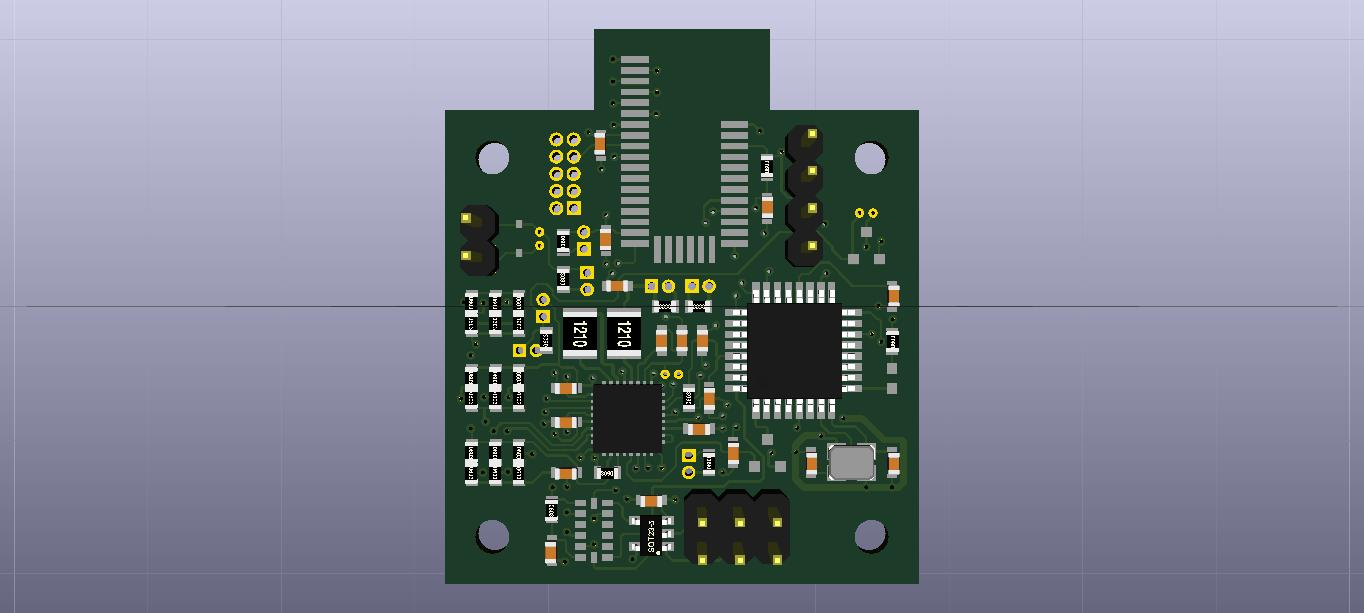
\includegraphics[height=6cm]{images/own_dwg/circuit/render.jpg}
  \end{center}
  \caption{\label{fig:pcb_render} Completed assembly of designed system.}
\end{figure}

The borders between sections are most clearly visible in the power planes of design shown in Figure \ref{fig:pcb_planes}. Power planes for each subcircuit have been separated for testing the current consumption, and therefore the outlines of the power planes follow the outlines of subcircuits.

\begin{figure}[htb]
  \begin{center}
    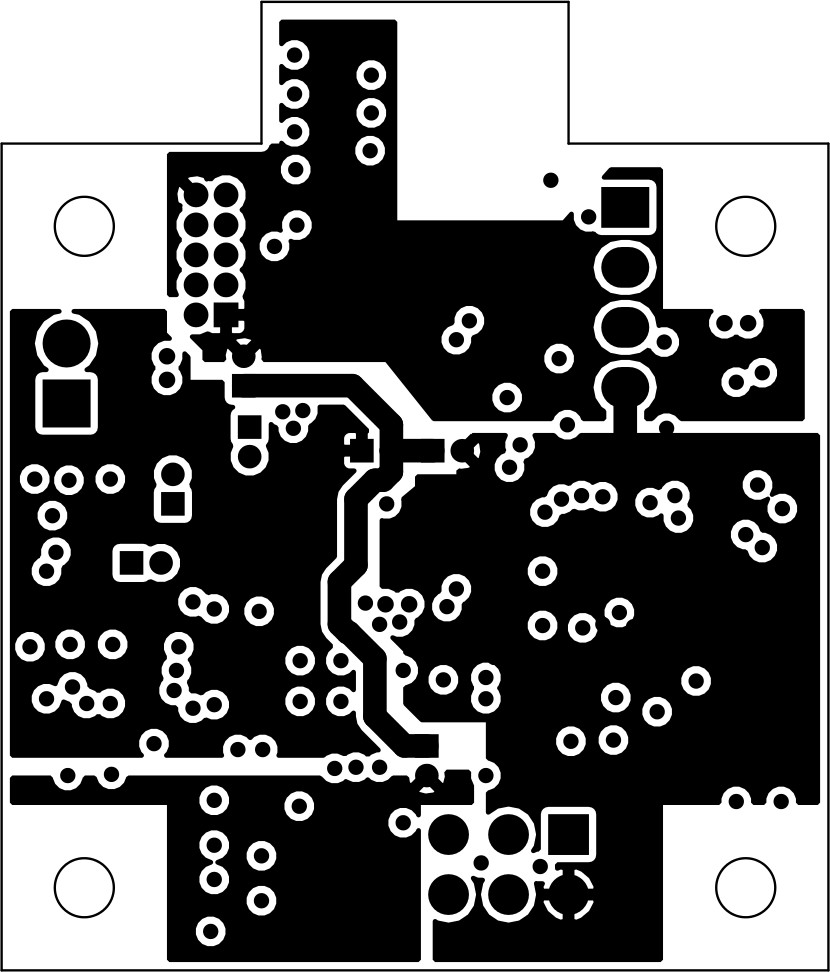
\includegraphics[height=6cm]{images/own_dwg/circuit/powerplane.jpg}
  \end{center}
  \caption{\label{fig:pcb_planes} Power planes of the PCB. Energy harvesting section is on left, control section is on right, radio communication is on top and accelerometer is on bottom.}
\end{figure}

In addition to mechanical and electrical properties, the PCB also acts as heat sink for mid-power components. In this circuit only LTC3331 needs consideration to thermal design. Circuit uses several vias under the pad of LTC3331 into the ground plane. As copper is an excellent conductor for heat, any thermal output from LTC3331 gets coupled to ground plane where it can spread to a wider area. Practically the expected milliwatt scale power in power supply section does not warrant concern for overheating.

Battery holder is the only large component in design where G-forces might cause a problem. The holder is on the backside of the PCB, where it can be mounted using adhesives or it can be supported by the harvester top.

\subsection{Mechanical design of the harvester}
This section details the mechanical considerations for both piezolectric and electromagnetic harvesters. First material options are explored, then the design for generators is presented.

Material for the generator has a few requirements. It has to have at least as good temperature characteristics as the magnet being used and it must be hard enough to not deform under impacts. Low friction coefficient is desirable as this leads to smaller  frictional losses, and long time durability under wear is of course desired. Being lightweight and easily machinable are also desired characteristics. As the generator is small, volumetric cost of the material is of little concern. For the electro-magnetic generator design material ferromagnetism has to be considered. Table \ref{parameters_of_materials} displays comparison of different materials considered for this application.

\begin{table}[htb]
%% Taulukon teksti
\caption{\label{parameters_of_materials} Materials for the shaft of the generator \cite{PlasticsInternational2015, Etra, Goodfellow, McCarr}.}
\begin{center}
\fbox{
\begin{tabular}{l l l l l l}
\textbf{Material}& 
\textbf{Hardness}& 
\textbf{Friction} & 
\textbf{Durability} & 
\textbf{Temperature}\\ \hline
PTFE(Teflon)      & Very low   & Lowest                      & Lowest    & -190... + 250 \degree C \\ 
Polycarbonate     & Very high  & High       & -         & -60... + 125 \degree C \\ 
PA 6 (Nylon)      & Low        & Medium                      & High      & -40... + 80 \degree C  \\ 
Oil-infused Nylon & Low        & Very low                    & Very high & -20... + 105 \degree C \\ 
Acryllic          & High       & -                           & -         & -40... + 70 \degree C \\ 
Polyacetal (POM C)& Medium     & Low                         & Low       & -50... + 105 \degree C \\ 
Carbon fiber     & Highest     & Highest                         & High       & ... + 80 \degree C \\ 
\end{tabular}
}

\end{center}
\end{table}

From the Table \ref{parameters_of_materials} it can be seen that there is no single best material for the harvester. Polycarbonate and carbon fibre have excellent mechanical strength but they have high friction. Teflon and nylon have lower friction, but they have poor mechanical rigidity. 

In the end acryllic was chosen as the material of the harvester. While acryllic is not a best material by any single metric, it has the necessary properties. Acryllic is easy to machine and readily available which were decisive factors for the selection of acrylic over other materials. 

As the minimum diameter of the harvester is defined by piezoelement diameter of 34 mm, both generators are designed with 35 mm square bases. Both generators also use same mounting hole pattern for electronics: 2.75 mm diameter holes at the corners of the square.

The generator was machined using slices of laser cut acrylic and standard acrylic tubing. The process is somewhat similar to 3D-printing, as several thin layers form up the final part. The acrylic parts used in generator are shown in Figure \ref{fig:lasercut}.

\begin{figure}[htb]
  \begin{center}
    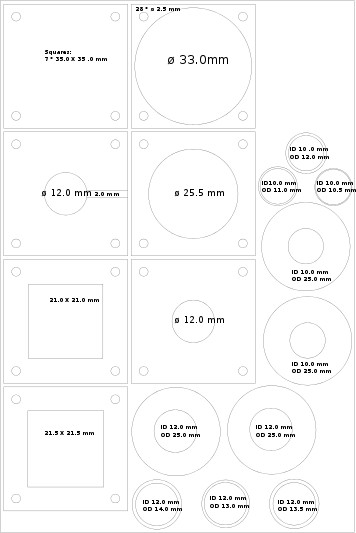
\includegraphics[height=15cm]{images/own_dwg/mechanical/layers.jpg}
  \end{center}
  \caption{\label{fig:lasercut} 150 * 150 mm sheet for laser cutting. Main structure is formed by squares with mounting holes. Squares have cutouts for pieces of generator, such as piezoelectric disk and stator magnets. Original idea was to make shaft of the generator out of laser cut rings, however process of laser cutting deformed thinner rings and alignment of the rings was not accurate enough for a smooth internal shaft required by rotor magnet.}
\end{figure}

While the initial approach for building the shaft of the generator was to use lasercut rings to form the shaft, the process of lasercutting warped thinner rings and mechanical alignment of the rings was difficult. Therefore a standard 10 mm inner diameter 12 mm outer diameter tube was selected as the shaft of electromagnetic harvester.

